
\documentclass[journal]{IEEEtran/IEEEtran}

\usepackage[utf8x]{inputenc}
\usepackage{cite}
\usepackage{hyperref}
\usepackage{url}
\usepackage{verbatim}
\usepackage{epstopdf}
\usepackage[pdftex]{graphicx}
\graphicspath{{img/}}
\DeclareGraphicsExtensions{.eps,.pdf,.png,.jpg,.jpeg}
\usepackage[cmex10]{amsmath}
\usepackage{array}
\usepackage{float}
\usepackage{color}
\usepackage[usenames,dvipsnames]{xcolor}
\usepackage{amssymb}

% correct bad hyphenation here
\hyphenation{op-tical net-works semi-conduc-tor}

\newcommand\ver[1]{%
{\texttt{#1}}}
\usepackage{listingsutf8}
\lstdefinelanguage{CSharp}
{
 morecomment = [l]{//}, 
 morecomment = [l]{///},
 morecomment = [s]{/*}{*/},
 morestring=[b]", 
 sensitive = true,
 morekeywords = {abstract,  event,  new,  struct,
   as,  explicit,  null,  switch,
   base,  extern,  object,  this,
   bool,  false,  operator,  throw,
   break,  finally,  out,  true,
   byte,  fixed,  override,  try,
   case,  float,  params,  typeof,
   catch,  for,  private,  uint,
   char,  foreach,  protected,  ulong,
   checked,  goto,  public,  unchecked,
   class,  if,  readonly,  unsafe,
   const,  implicit,  ref,  ushort,
   continue,  in,  return,  using,
   decimal,  int,  sbyte,  virtual,
   default,  interface,  sealed,  volatile,
   delegate,  internal,  short,  void,
   do,  is,  sizeof,  while,
   double,  lock,  stackalloc,   
   else,  long,  static,   
   enum,  namespace,  string}
}
\lstset{
	tabsize=4,
	basicstyle={\ttfamily \footnotesize},
	identifierstyle={\ttfamily},
	inputencoding=cp1250,
	%barvanje kode
	commentstyle={\sffamily \color[rgb]{0,0.5,0}},
	stringstyle=\color[rgb]{0.5,0,1},
	keywordstyle=\color[rgb]{0,0,1},
	%barvanje kode
	%language=JavaScript,
	%iz source datotek potegnemo tisto med //@begin@ ...koda... //@end@
	%rangeprefix={\#@},
	%rangesuffix={@},
	%linerange=begin-end,
	%includerangemarker=false,
	%lomljenje predolgih vrstic
	tabsize=2, 
	breaklines=true,
	showstringspaces=false,
	prebreak=\raisebox{0ex}[0ex][0ex]{\ensuremath{\hookleftarrow}},
	%okvir
	%frame=single,
	%frameround={t}{t}{t}{t},
	%numbers=left,
	%firstnumber=1,
	%framexleftmargin=19pt,
	%xleftmargin=23pt,
	xrightmargin=4pt,
	framerule=0pt
	%številčenje
}

\newcommand\subsect[1]{\subsection{#1}\noindent}
\newcommand\tab[0]{{\color{white}.}\ \ \ \ }

\begin{document}
\title{Weka on .NET}

\author{Matic~Potočnik, Gregor~Majcen}%
%\thanks{M. Shell is with the Department
%of Electrical and Computer Engineering, Georgia Institute of Technology, Atlanta,
%GA, 30332 USA e-mail: (see http://www.michaelshell.org/contact.html).}% <-this % stops a space
%\thanks{J. Doe and J. Doe are with Anonymous University.}% <-this % stops a space
%\thanks{Manuscript received April 19, 2005; revised January 11, 2007.}}

\markboth{FRI MLDM Workshop 2012}{}
%\IEEEspecialpapernotice{(Invited Paper)}

\maketitle

\begin{abstract}
This paper will describe and benchmark several approaches to using Weka on the .NET Framework.
\end{abstract}

\begin{IEEEkeywords}
Weka, .NET, benchmark, machine learning.
\end{IEEEkeywords}

\IEEEpeerreviewmaketitle

\section{Introduction}
\IEEEPARstart{T}{his} paper will provide the reader with an overview and performance notes on using the Weka data-mining library\cite{weka:2009} on the Microsoft .NET framework. Weka originally runs on the Java Virtual Machine (JVM), but there are methods which allow running Java code on .NET. This paper will describe several approaches and benchmark the performance of each approach on multiple machine learning algorithms. We will also list some possible use-cases of Weka on .NET. For a brief description of the technologies used, see Appendix \ref{Tools}.\\

\hfill \today
\ \\ \ \\
\textbf{Note:}\\
The complete source code and most files, which were used while creating this paper, are available online at:\\ \url{https://github.com/HairyFotr/Weka-on-.NET}\\
\section{Java on .NET}
In this section we will describe a few methods for using Java code on the .NET Framework. The text presumes usage of Microsoft Windows and that Java JDK, .NET Framework, Weka, IKVM, C\# and F\# compiler and Mono are already installed and that the correct directories have been added to the system PATH.\\ \ \\
The exact versions of software used for generating the results in this paper are:
\begin{itemize}
\item Microsoft Windows 7 Professional x64
\item Java 1.6.0\_26
\item Microsoft.NET Framework v4.0.30319
\item Weka 3.6.6
\item Microsoft Visual C\# 2010 Compiler 4.0.30319.1
\item Microsoft F\# Compiler 2.0.0.0
\item IKVM 0.46.0.1
\item Mono 2.10.8
\end{itemize}
\subsect{IKVM directly running Java code on .NET}This approach is the simplest if we just want to run Java on the .NET Framework, but its practical use is somewhat questionable as you cannot mix Java and .NET code this way. That means you cannot use any of the .NET libraries and code. But if you have the .class files precompiled you can run them on .NET without having Java installed on your system.

All the user needs to do to use this approach is to use the command-line command \ver{ikvm} instead of \ver{java} when running a program from the console. IKVM automatically accepts and uses additional Java libraries and no additional action is needed.
\begin{lstlisting}[title={Weka example}]
  javac -cp weka.jar;. Program.java
  ikvm -cp weka.jar;. Program 
\end{lstlisting}
The \ver{ikvm} command accepts all the command-line switches \ver{java} does, but some don't necessary do anything. For instance -- memory switches such as \ver{-xmx1024m} get ignored, as the .NET handles memory differently and does not hard-limit heap space the same way the JVM does. IKVM alerts us if some option is ignored or unsupported.

\subsect{Using a IKVM-generated .dll with .NET/Mono}For this approach we need a Java library inside a \ver{.jar} package. We can then proceed to generate a \ver{.dll} library using \ver{ikvmc}. The \ver{ikvmc} command has several options, but the most important for our use is the \ver{-target} parameter, which can take the following values:
\begin{itemize}
\item \textbf{exe} -- generates an .exe that runs in a command window
\item \textbf{winexe} -- generates an .exe for GUI applications
\item \textbf{library} -- generates a .dll
\item \textbf{module} -- generates a .netmodule
\end{itemize}
We are going to use the \ver{library} value, which generates a .dll which can then be referenced by .NET Framwork and Mono code. In C\# programs we use the \ver{using} directive and the \ver{open} directive is used in F\#.
\begin{lstlisting}[title={Weka example}]
  ikvmc -target:library weka.jar
\end{lstlisting}
After \ver{ikvmc} has generated the .dll for us, we can use Visual Studio or the command-line compiler to compile our program with the .dll.
\begin{lstlisting}[title={Weka example (.NET)}]
  csc Program.cs -r:weka.dll,IKVM.OpenJDK.Core.dll,IKVM.Runtime.dll
  Program.exe
\end{lstlisting}
\begin{lstlisting}[title={Weka example (Mono)}]
  dmcs Program.cs -r:weka.dll,IKVM.OpenJDK.Core.dll,IKVM.Runtime.dll
  mono Program.exe
\end{lstlisting}

\subsect{Using WekaSharp on .NET/Mono}Here a pre-built F\# wrapper around Weka is used. It also uses IKVM, but there is also some native F\# code, which simplifies Weka programming in F\#. In this paper we've used Weka directly with the Weka.dll provided with WekaSharp, and didn't explore the options and benefits the wrapper provides.
\begin{lstlisting}[title={Weka example (F\#)}]
  fsc Program.fsx -r:weka.dll -r:IKVM.OpenJDK.Core.dll -r:IKVM.Runtime.dll
  Program.exe
\end{lstlisting}


\section{Benchmarking}
In this section we will discuss the benchmarking setup and methods used to generate the results.
\subsect{Overview}We will use the following Weka algorithms:
\begin{itemize}
\item weka.classifiers.bayes.NaiveBayes
\item weka.classifiers.trees.RandomForest
\item weka.classifiers.trees.J48
\item weka.classifiers.rules.ConjunctiveRule
\item weka.classifiers.functions.MultilayerPerceptron
\item weka.classifiers.functions.SMO
\end{itemize}\ \\
%The following datasets:
%\begin{itemize}
%\item ReutersCorn (included with Weka)
%\item ReutersGrain (included with Weka)
%\item ??? (provided by ???) TODO
%\end{itemize}\ \\
Measurements will be made for these languages/platforms:
\begin{itemize}
\item \textbf{java} -- Java with Weka.jar
\item \textbf{javaikvm} -- Java with Weka.jar on .NET via IKVM
\item \textbf{net} -- C\# with IKVM-generated Weka.dll on .NET
\item \textbf{mono} -- C\# with IKVM-generated Weka.dll on Mono
\item \textbf{fsharp} -- F\# with WekaSharp's Weka.dll on .NET
\end{itemize}

\subsect{Benchmarking code}For benchmarking purposes, a functionally equivalent short benchmarking program was written in Java, C\# and F\#.
\lstinputlisting[title={\footnotesize Benchmark (pseudocode)}]{src/Program.txt}
The only difference between implementations, that is worth noting was the use of \ver{System.nanoTime()} in Java and the \ver{Stopwatch} class in C\# and F\# for measuring time, but we've tested both approaches on .NET and found that there is no noticeable difference.

\subsect{Code correctness}One of the concerns we had was whether or not the Weka library behaviour was still the same on .NET, as it was on the JVM, and also if our programs were really equivalent.

To test this we ran all the programs and checked if the classification accuracy is the same on all three. The test was run on all the selected algorithms. Below is a sample output of one of these runs. As you can see there are some additional trailing zeroes with the last line, which is the F\# output, but as we've discovered this was due to typing, not due to numerical error. The other examples remained of the type \ver{java.lang.Float}, but F\# has a different type-sytem, which raised a type-error when doing arithmetic with mixed types, so we had to cast the numbers to F\#'s \ver{float} type which has a slightly different behaviour when converting float to string. Also, this difference appears in the calculation of the percentage -- the classification results are exactly the same on all runs and so we have concluded that the code is correct.
\lstinputlisting[breaklines=false,basicstyle={\ttfamily \scriptsize},title={\footnotesize Sample output}]{res/correctness.txt}

\subsect{Benchmarking script}To simplify and speed-up the benchmarking process we have constructed a script which runs all the benchmarks and saves the results into a file. The script was written in Windows Batch. The script allowed us to set the number of runs, desired algorithms, the name of the dataset and which languages/platforms are included in the benchmarked.

\lstinputlisting[title={\footnotesize Benchmarking script (pseudocode)}]{src/test.txt}
The script outputs the results in a format that is useful almost as-is in Mathematica for further analysis and graph plotting. Here is an example of a small Java run:
\lstinputlisting[title={\footnotesize Result sample}]{res/smallresult.txt}


\section{Results}
In this section we will present the benchmarking results.
\subsect{Dataset}We used a bioinformatics dataset which was used as a part of a challenge/homework in an bioinformatics class on FRI\cite{citation needed}. The dataset was in CSV format (Comma-Separated Values), and Weka uses the ARFF (Attribute-Relation File Format), so we used an online CSV to ARFF converter to convert it into an appropriate format. We then then took a sample of only 500 rows from the training data. This was done because some machine-learning algorithms, such as SMO and MultilayerPerceptron, don't work well with multi-valued attributes, and we wished to run all classifiers on the same dataset. The testing data on which we executed the classification was 100000 rows long. Here is the ARFF header of the dataset in question:
\lstinputlisting[title={\footnotesize Dataset header}]{src/datasetheader.txt}

\subsect{Joint results}We will begin the presentation of the results with the graph of the total time for all algorithms. We ran the benchmark 10 times on the above dataset for each of the algortihms and each of the language/platform combinations.
\begin{figure}[H]
\centering
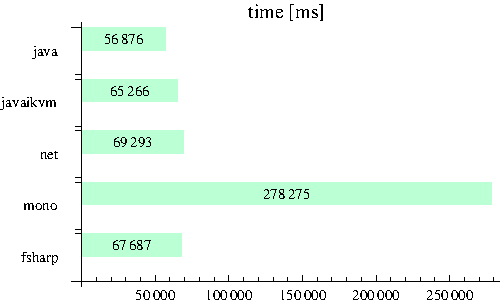
\includegraphics[width=3.5in]{total}
\caption{Joint results}
\end{figure}
As we can see from the graph Java is the fastest, the programs on .NET Framework ran at aproximately the same speed, and the program ran on Mono was several times slower.
\ \\ \ \\
Next we will look at the joint performance across all algorithms for reading, classifier building and classifier execution.
\begin{figure}[H]
\centering
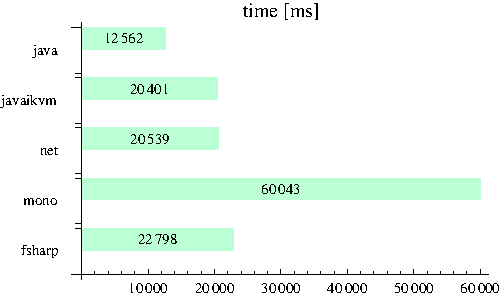
\includegraphics[width=3.5in]{read}
\caption{Reading performance results}
\end{figure}

\begin{figure}[H]
\centering
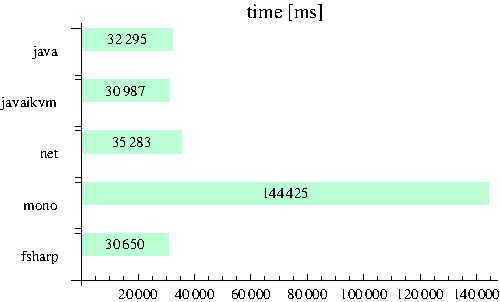
\includegraphics[width=3.5in]{build}
\caption{Classifier building performance results}
\end{figure}

\begin{figure}[H]
\centering
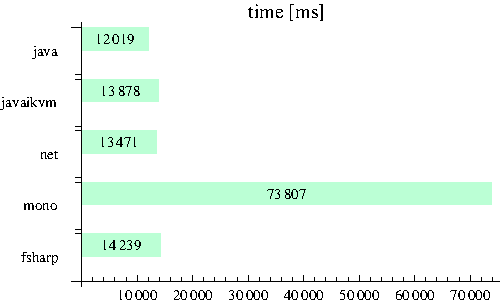
\includegraphics[width=3.5in]{classify}
\caption{Classifier execution performance results}
\end{figure}
\subsect{Results by algoritm}
In this subsection we will present the performance results for each algorithm, separately.\\ \ \\
We have used the following colors:
\definecolor{orange}{rgb}{1,0.86,0.66}
\definecolor{green}{rgb}{0.73,1,0.83}\\
\tab {\color{orange} $\blacksquare$} -- classifier building time\\
\tab {\color{green} $\blacksquare$} -- classifier exectuion time\\
\begin{figure}[H]
\centering
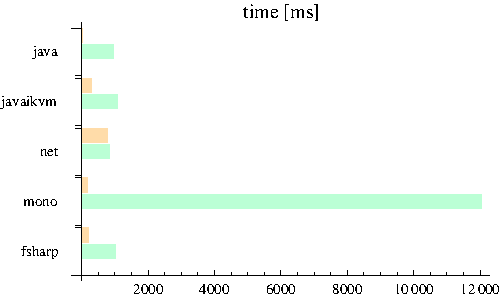
\includegraphics[width=3.5in]{NaiveBayes}
\caption{NaiveBayes performance results}
\end{figure}
\begin{figure}[H]
\centering
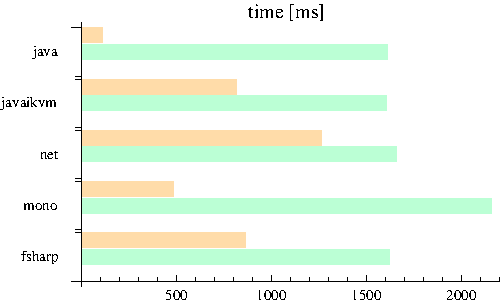
\includegraphics[width=3.5in]{RandomForest}
\caption{RandomForest performance results}
\end{figure}
\begin{figure}[H]
\centering
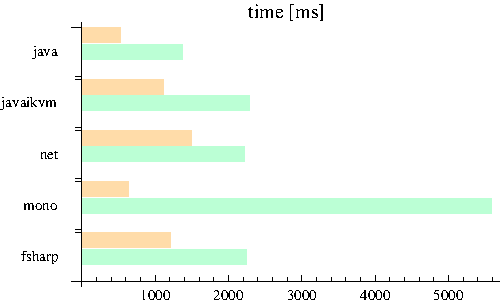
\includegraphics[width=3.5in]{SMO}
\caption{SMO performance results}
\end{figure}
\begin{figure}[H]
\centering
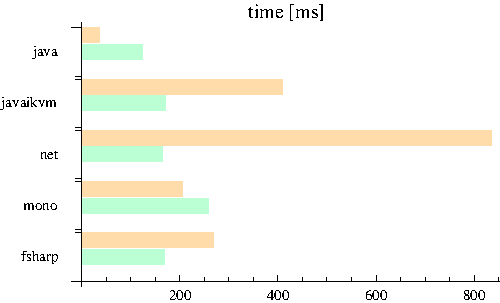
\includegraphics[width=3.5in]{J48}
\caption{J48 performance results}
\end{figure}
\begin{figure}[H]
\centering
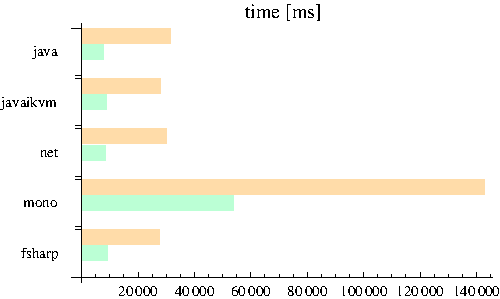
\includegraphics[width=3.5in]{MultilayerPerceptron}
\caption{MultilayerPerceptron performance results}
\end{figure}
\begin{figure}[H]
\centering
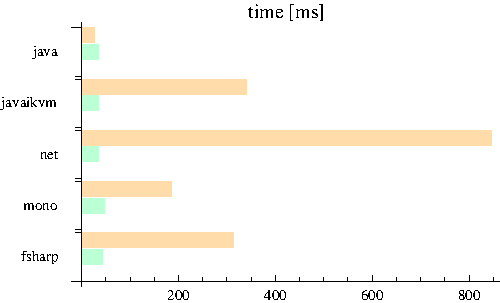
\includegraphics[width=3.5in]{ConjunctiveRule}
\caption{ConjunctiveRule performance results}
\end{figure}
\subsect{Memory usage}
One aspect of performance is also the memory usage of the programs. The memory benchmark was performed simply by stopping the programms right before their ending (this was done by adding a \ver{readLine} command to the end of all three programs), and then writting down the \ver{Memory - Peak Working Set} figure from the Windows Task Manager.
\begin{figure}[H]
\centering
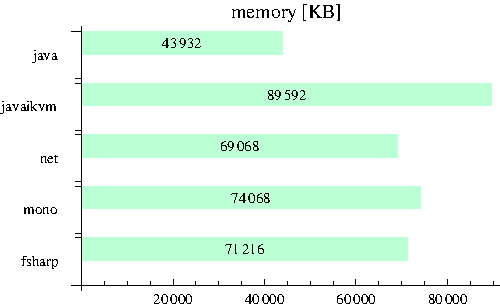
\includegraphics[width=3.5in]{res/mem}
\caption{Memory performance results}
\end{figure}
The result shown above was produced by building and executing all of the selected algorithms once. The benchmark was repeated a few times, but there was less than 1MB difference in memory usage between runs.

% Note that IEEE typically puts floats only at the top, even when this
% results in a large percentage of a column being occupied by floats.
%\begin{figure}[!t]
%\centering
%\includegraphics[width=2.5in]{myfigure}
% where an .eps filename suffix will be assumed under latex, 
% and a .pdf suffix will be assumed for pdflatex; or what has been declared
% via \DeclareGraphicsExtensions.
%\caption{Simulation Results}
%\label{fig_sim}
%\end{figure}

% An example of a double column floating figure using two subfigures.
% (The subfig.sty package must be loaded for this to work.)
% The subfigure \label commands are set within each subfloat command, the
% \label for the overall figure must come after \caption.
% \hfil must be used as a separator to get equal spacing.
% The subfigure.sty package works much the same way, except \subfigure is
% used instead of \subfloat.
%
%\begin{figure*}[!t]
%\centerline{\subfloat[Case I]\includegraphics[width=2.5in]{subfigcase1}%
%\label{fig_first_case}}
%\hfil
%\subfloat[Case II]{\includegraphics[width=2.5in]{subfigcase2}%
%\label{fig_second_case}}}
%\caption{Simulation results}
%\label{fig_sim}
%\end{figure*}
%
% Note that often IEEE papers with subfigures do not employ subfigure
% captions (using the optional argument to \subfloat), but instead will
% reference/describe all of them (a), (b), etc., within the main caption.


% An example of a floating table. Note that, for IEEE style tables, the 
% \caption command should come BEFORE the table. Table text will default to
% \footnotesize as IEEE normally uses this smaller font for tables.
% The \label must come after \caption as always.
%
%\begin{table}[!t]
%% increase table row spacing, adjust to taste
%\renewcommand{\arraystretch}{1.3}
% if using array.sty, it might be a good idea to tweak the value of
% \extrarowheight as needed to properly center the text within the cells
%\caption{An Example of a Table}
%\label{table_example}
%\centering
%% Some packages, such as MDW tools, offer better commands for making tables
%% than the plain LaTeX2e tabular which is used here.
%\begin{tabular}{|c||c|}
%\hline
%One & Two\\
%\hline
%Three & Four\\
%\hline
%\end{tabular}
%\end{table}

\section{Conclusion}
The results of the total classifier building performance were a bit of a surprise, as \ver{javaikvm} and \ver{fsharp} are actually faster than \ver{java}. Later results on particular classifiers showed that the benchmark was skewed by the MultilayerPerceptron benchmark, which accounted for more than half of the total benchmarking time. Another abnormality was Mono -- its performance was so bad, that it made some graphs hard to read. Here is the total graph again, with the MultilayerPerceptron and Mono results left out.
\begin{figure}[H]
\centering
\includegraphics[width=3.5in]{TotalTotal}
\caption{Total performance results}
\end{figure}

The results show that Java is the fastest by about 60\%, and the memory benchmarks also show about 60\% lower memory usage. Based on these results we conclude that using Weka on the .NET Framework is indeed possible and for some use-cases practical.

\section{Further work}
More algorithms and different datasets could be tested -- this paper doesn't include any regressional algoritms, and some algorithms used were not a good match for the dataset used. Weka also includes algorithms for preprocessing and filtering which were not featured here. The resulting data should also be weighted before being plotted, to avoid the skew in data that manifested itself here. We should also investigate how it was possible for .NET to be faster than Java in the MultilayerPerceptron benchmark, and why Mono performance was so bad in some cases.

Another thing which could be added are possible use-cases for Weka on .NET, such as using tools only available in the .NET ecosystem. Microsoft SQL server with its Analysis Services is a good example of a such tool\cite{sqlas:2012}.
\begin{thebibliography}{1}

\bibitem{weka:2009}
Mark Hall, Eibe Frank, Geoffrey Holmes, Bernhard Pfahringer, Peter Reutemann, Ian H. Witten (2009); The WEKA Data Mining Software: An Update; SIGKDD Explorations, Volume 11, Issue 1.
\bibitem{sqlas:2012}
David Hrovat (2012); Data Analysis with Microsoft SQL Server 2008 R2 Analysis Services; FRI MLDM Workshop 2012

\end{thebibliography}

\newpage

% if have a single appendix:
%\appendix[Proof of the Zonklar Equations]
% or
%\appendix  % for no appendix heading
% do not use \section anymore after \appendix, only \section*
% is possibly needed
\appendices
\section{Tools}\label{Tools}
In this appendix section we will briefly describe some of the technologies and tools we've used.

\subsect{Weka}Weka (Waikato Environment for Knowledge Analysis) is a widely used machine learning library, both in academia and business. 
\begin{figure}[H]
\centering
\includegraphics[width=2.2in]{weka}
\caption{Weka logo}
\label{fig_sim}
\end{figure}
Its development started in 1993 at the University of Waikato, New Zealand. Initially it was written in TCL/TK and C, but later in 1997 it was completely rewritten in Java. Weka is free software released under the GNU General Public License.

%Weka is distributed as a single \verb .jar file, which can be either used as a library or run as an data-mining application called Weka workbench.

\subsect{Mono}Mono is a software platform designed to allow developers to easily create cross platform applications. Mono is an open-source implementation of Microsoft's .NET Framework based on the ECMA standards for C\# and the Common Language Runtime (CLI).
\begin{figure}[H]
\centering
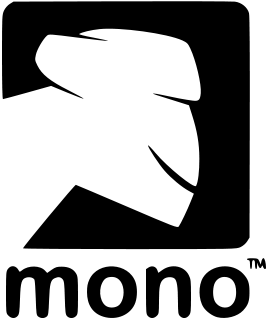
\includegraphics[width=1.25in]{Mono}
\caption{Mono logo}
\label{fig_sim}
\end{figure}

\subsect{IKVM}IKVM.NET is an implementation of Java for both Mono and the Microsoft .NET Framework. It includes the following components:
\begin{itemize}
\item A Java Virtual Machine implemented in .NET
\item A .NET implementation of the Java class libraries
\item Tools that enable Java and .NET interoperability
\end{itemize}
\begin{figure}[H]
\centering

\includegraphics[width=2in]{IKVM}
\caption{IKVM logo}
\label{fig_sim}
\end{figure}


%\section*{Acknowledgment}
%We would like to thank our mentor Matjaž Kukar.

% trigger a \newpage just before the given reference
% number - used to balance the columns on the last page
% adjust value as needed - may need to be readjusted if
% the document is modified later
%\IEEEtriggeratref{8}
% The "triggered" command can be changed if desired:
%\IEEEtriggercmd{\enlargethispage{-5in}}

% references section

% can use a bibliography generated by BibTeX as a .bbl file
% BibTeX documentation can be easily obtained at:
% http://www.ctan.org/tex-archive/biblio/bibtex/contrib/doc/
% The IEEEtran BibTeX style support page is at:
% http://www.michaelshell.org/tex/ieeetran/bibtex/
%\bibliographystyle{IEEEtran}
% argument is your BibTeX string definitions and bibliography database(s)
%\bibliography{IEEEabrv,../bib/paper}
%
% <OR> manually copy in the resultant .bbl file
% set second argument of \begin to the number of references
% (used to reserve space for the reference number labels box)


% biography section
% 
% If you have an EPS/PDF photo (graphicx package needed) extra braces are
% needed around the contents of the optional argument to biography to prevent
% the LaTeX parser from getting confused when it sees the complicated
% \includegraphics command within an optional argument. (You could create
% your own custom macro containing the \includegraphics command to make things
% simpler here.)
%\begin{biography}[{\includegraphics[width=1in,height=1.25in,clip,keepaspectratio]{mshell}}]{Michael Shell}
% or if you just want to reserve a space for a photo:
\begin{comment}
\newpage

\begin{IEEEbiography}[{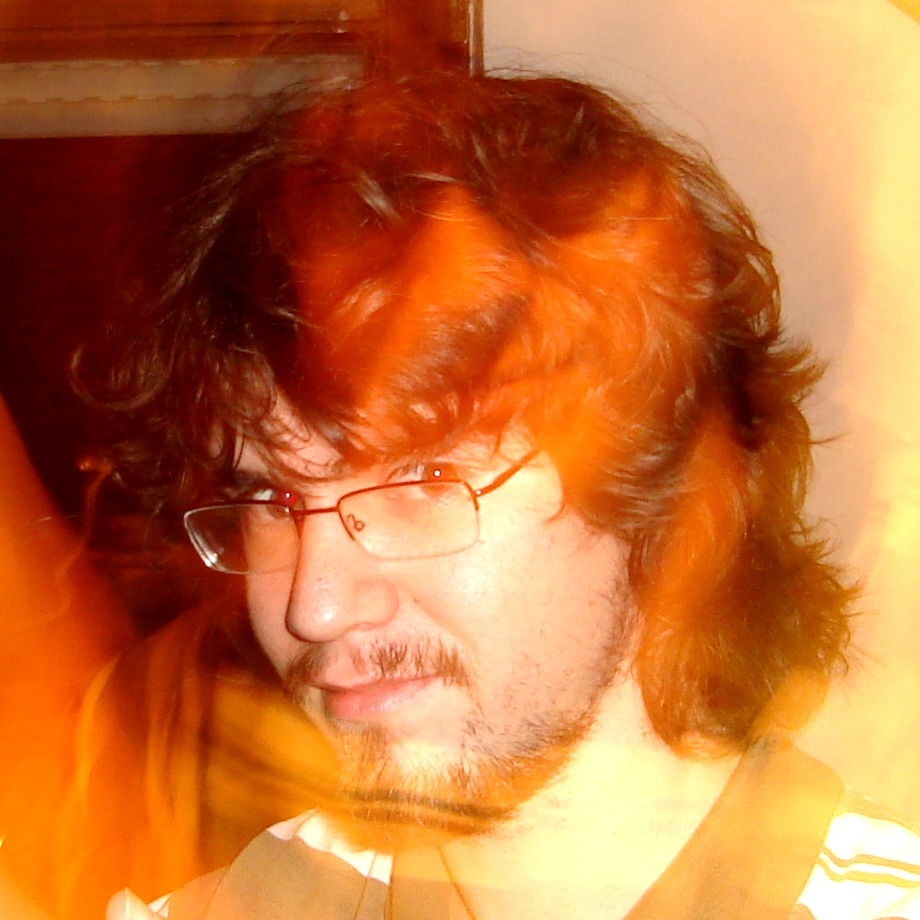
\includegraphics[width=1in,height=1.25in,clip,keepaspectratio]{matic}}]{Matic Potočnik}
Biography text here.
\end{IEEEbiography}

% if you will not have a photo at all:
\begin{IEEEbiography}{Gregor Majcen}
Biography text here.
\end{IEEEbiography}

% You can push biographies down or up by placing
% a \vfill before or after them. The appropriate
% use of \vfill depends on what kind of text is
% on the last page and whether or not the columns
% are being equalized.

%\vfill

% Can be used to pull up biographies so that the bottom of the last one
% is flush with the other column.
%\enlargethispage{-5in}

\end{comment}
\end{document}


